\documentclass[xcolor={dvipsnames}, handout]{beamer}
%\documentclass[xcolor={dvipsnames}]{beamer}
%\usepackage{amsmath,amsfonts,amssymb,pxfonts,eulervm,xspace}
\usepackage{amsmath, amsfonts, amssymb, mathtools, eulervm, xspace}
\usepackage{bm}
\usepackage{mathrsfs} % math script fonts
\usepackage{tikz}
\newtheorem{prop}{Proposition} %math?

\usetikzlibrary{cd} % commutative diagrams
\usepackage{subcaption} % subfigure float captioning

\usepackage{tabulary}
\usepackage{tabularx}
\usepackage{booktabs}
\usepackage{multirow}

\usepackage{graphicx}

\usepackage{appendixnumberbeamer} 
\usepackage{comment}
\usepackage{minted}
\setminted[python]{fontsize=\scriptsize, 
                   linenos,
                   numbersep=8pt,
                   autogobble, 
                   frame=lines,
                   bgcolor=bg,
                   framesep=3mm} 
\usepackage{notation} % move this later

\graphicspath{.figures/}

\usepackage[backend=bibtex, style=alphabetic, sorting=none, doi=false,isbn=false,url=false, giveninits=true]{biblatex}
\bibliography{../draft/glasslab_viz.bib}

\usetheme{ccnycrest}

\newenvironment{changemargin}[2]{%
\begin{list}{}{%
\setlength{\topsep}{0pt}%
\setlength{\leftmargin}{#1}%
\setlength{\rightmargin}{#2}%
\setlength{\listparindent}{\parindent}%
\setlength{\itemindent}{\parindent}%
\setleng{}th{\parsep}{\parskip}%
}%
\item[]}{\end{list}}

\begin{document}

\title{Topological Equivariant Artist Model}

\begin{frame}
	\titlepage
    Hannah Aizenman\\
    Advisor: Dr. Michael Grossberg \\
    Committee: Dr. Robert Haralick, Dr. Lev Manovich, Dr. Huy Vo\\
    External Member: Dr. Marcus Hanwell
\end{frame}

\section{Introduction}

\begin{frame}{Visualizations are structure preserving maps}
    %add arrow between data and vizualizations
    % we're focused on building good arrows 
    \begin{figure}
        \includegraphics[width=\textwidth]{figures/intro/viz_same.png}
    \end{figure}
    \pause 
    \begin{description}
        \item[equivariance] properties of data and visual encoding match
    \pause 
        \item[continuity] connectivity of data and visual encoding match
    \end{description}
\end{frame}

\begin{frame}{Domain specific libraries assume data structure\cite{HeerSoftware2006}}
    \begin{table}
        %\renewcommand{\arraystretch}{2}
        \begin{tabulary}{\textwidth}{|L|l|l|}\toprule
            \includegraphics[width=.24\textwidth]{figures/intro/table.png} & \includegraphics[width=.3\textwidth]{figures/intro/landsat.png} & \includegraphics[width=.33\textwidth]{figures/math/graph.png} \\
            ggplot\cite{wickhamGgplot2ElegantGraphics2016a}  & ImageJ\cite{schneiderNIHImageImageJ2012}& Gephi\cite{bastianGephiOpenSource2009}\\
            Vega\cite{satyanarayanDeclarativeInteractionDesign2014} & ImagePlot\cite{studiesCulturevisImageplot2021} & Graphviz\cite{ellsonGraphvizOpenSource2002}\\
            Altair\cite{vanderplasAltairInteractiveStatistical2018}& Napari\cite{nicholas_sofroniew_2021_4533308} & Networkx\cite{HagbergExploringNetwork2008}\\
             Tableau\cite{StoltePolaris2002,hanrahanVizQL2006,MackinlayShowme2007} & &\\
             \bottomrule
        \end{tabulary}
    \end{table}
\end{frame}


\begin{frame}{General purpose libraries can't\cite{toryRethinkingVisualizationHighlevel2004}}
    \begin{figure}
        \includegraphics[height=.5\textheight]{figures/intro/dataset_diagram.png}
        \caption{Data Representation, MayaVi 4.7.2 docs\cite{DataRepresentationMayavi}}
    \end{figure}
    \begin{enumerate}
        \item Matplotlib\cite{hunterMatplotlib2DGraphics2007} $\rightarrow$Seaborn\cite{waskom2020seaborn}, xarray \cite{hoyer2017xarray} 
        \item D3 \cite{bostockDataDrivenDocuments2011}
        \item VTK \cite{hanwellVisualizationToolkitVTK2015,geveci2012vtk}(MayaVi\cite{RamachandranMayaVI2011})$\rightarrow$ Titan\cite{brianwylieUnifiedToolkitInformation2009}, ParaView\cite{ahrens2005paraview}
    \end{enumerate}
\end{frame}

\begin{frame}{Best practices in visualization design}
    \begin{description}
        \item[Expressiveness] structure preserving mappings\cite{mackinlayAutomatingDesignGraphical1986}
        \pause
        \item[Naturalness] easier to understand when properties match\cite{norman_things_smart}
        \pause
       \item[Graphical Integrity] graphs show \textbf{only} the data\cite{tufteVisualDisplayQuantitative2001}
    \end{description}
\end{frame}

\subsection{Contributions}
\begin{frame}{Contributions}
    \begin{description}
        \item[Topological] continuity  
        \item[Equivariant] monoid action 
        \item[Artist] Matplotlib $\textit{artist}: \textit{data} \rightarrow \textit{graphic}$ 
        \item [Model] 
    \end{description}
\end{frame}


\section{Mathematical Framework}

\begin{frame}{Topological Equivariant Artist Model}
    \centering
    An artist $\mathscr{\vartist}$ is an equivariant map 
    \begin{equation*}\Huge
        \mathscr{\vartist}: \mathscr{\dtotal} \rightarrow \mathscr{\gtotal}
    \end{equation*}
    from data $\mathscr{\dtotal}$ space to graphic $\mathscr{\gtotal}$ space. 
\end{frame}


\subsection{Data Model}
\begin{frame}{Model data as a fiber bundle \cite{butlerVectorBundleClassesForm1992,butlerVisualizationModelBased1989}}
    A fiber bundle is a tuple $(\dtotal,\,\dbase,\,\pi ,\,\dfiber)$ defined by the map $\pi$
    \begin{equation*}
        \label{eq:fiber_bundle}
        \begin{tikzcd}[ampersand replacement=\&]
            \dfiber \arrow[r, hook] \& \dtotal \arrow[r, "\pi"] \& \dbase
        \end{tikzcd}
    \end{equation*}
    \begin{description}
        \pause
        \item[total space \dtotal] dataset topology
        \pause
        \item[fiber space \dfiber] variable schema
        \pause
        \item[base space \dbase] continuity
    \end{description}
\end{frame}

\begin{frame}{Encode variable types in a schema like fiber \cite{spivakDatabasesAreCategories2010,spivakSIMPLICIALDATABASES}}
    \begin{figure}[H]
        \centering
        \includegraphics[width=\textwidth]{figures/math/fiber.png}
    \label{fig:data_fiber_example}
    \end{figure}
\end{frame}

\begin{frame}{Structure of components of \dfiber}
    \begin{figure}[H]
        \centering
        \includegraphics[height=.3\textheight]{figures/math/fiber.png}
    \label{fig:data_fiber_example}
    \end{figure}
        \begin{equation*}
            \dfiber = \dfiber_0 \times \ldots \times \dfiber_i \times \ldots \times \dfiber_n
        \end{equation*}
        \pause
        Monoid actions $\monoid_{i}$ (e.g. rotation, partial ordering) define the structure on $\dfiber_i$
        \begin{equation*}
            \bullet: \monoid_i\times \dfiber_i \rightarrow \dfiber_i
        \end{equation*}
        They must be associative and have an identity element. 
\end{frame}


\begin{frame}{\dbase\ is an indexing space}
    \begin{figure}[H]
        \includegraphics[width=1\textwidth]{figures/math/base.png}
    \label{fig:base_example}
    \end{figure}
\end{frame}

\begin{frame}{Structural \textit{keys} with associated \textit{values} \cite{munznerVisualizationAnalysisDesign2014}}
\begin{figure}
    \includegraphics[width=1\textwidth]{figures/intro/munzner_datatypes.png}
    \caption{Figure 2.8 in Munzner's Visualization Analysis and Design\cite{munznerVisualizationAnalysisDesign2014}}
\end{figure}
\pause
\begin{figure}[H]
    \includegraphics[width=.5\textheight]{figures/math/base.png}
    \label{fig:base_example}
\end{figure}
\end{frame}


\begin{frame}{Data are sections \dsection\ on \dtotal}
    For any fiber bundle, there exists a map
    \begin{equation*}
        \begin{tikzcd}[ampersand replacement=\&]
            \dfiber \arrow[r, hook] \& \dtotal \arrow[d, "\pi"'] \\
                              \& \dbase \arrow[u, "\dsection"', bend right]
        \end{tikzcd}
    \end{equation*}
     s.t. $\pi(\dsection(\dbasepoint)) = \dbasepoint$. $\Gamma(\dtotal)$ is the set of all global sections.
     \begin{figure}[H]
        \includegraphics[width=1\linewidth]{figures/math/fiberbundle.png}
        \label{fig:data_sections}
    \end{figure}
\end{frame}


\subsection{Graphics}
\begin{frame}{Graphic Bundle $(\gtotal,\,\gbase,\,\pi ,\,\gfiber)$} % watch dr explaination
    Continuity is preserved via the many \gbasepoint\ to one \dbasepoint\ map $\vindex: \gbase\rightarrow\dbase$
    \begin{equation*} 
        \begin{tikzcd}[ampersand replacement=\&]
            F \arrow[r, hook] \& E \arrow[d, "\pi"']              \& D \arrow[r, hook] \& H \arrow[d, "\pi"']                                 \\
                              \& K \arrow[u, "\tau"', bend right] \&                   \& S \arrow[ll, "\xi"'] \arrow[u, "\rho"', bend right]
            \end{tikzcd}
        \end{equation*}
    \pause
    \gfiber\ is a proxy for the target display, for example $(x,\, y,\, r,\, g,\, b) \in \gfiber$
    \pause
    \begin{figure}[H] %%%bring up one at a time
        \includegraphics[width=1\textwidth]{figures/math/retraction_maps.png}
        \label{fig:graphic_retraction_map}
    \end{figure}
\end{frame}

\subsection{Artist}%formalize the structure
\begin{frame}{Visual bundle $(\vtotal,\,\dbase,\,\pi ,\,\vfiber)$}
\begin{equation*}
    \label{eq:artist_diagram}
    \begin{tikzcd}[ampersand replacement=\&]
        \dtotal^{\prime} \arrow[r, "\vchannel"] \arrow[rd, "\pi"'] \& \vtotal \arrow[d, "\pi"] \& \vindex^*\vtotal \arrow[r, "\vmark"] \arrow[d, "\vindex^*\pi"'] \arrow[l, "\vindex^*"'] \& \gtotal \arrow[ld, "\pi"] \\
                                              \& \dbase                  \& \gbase \arrow[l, "\vindex"']                                              \&                    
        \end{tikzcd}
\end{equation*}
\pause
\begin{equation*}
    \mathcal{A}:\mathcal{E}\rightarrow\mathcal{E}
\end{equation*}
\pause
The topological artist is a sheaf map
\begin{equation*}
    \vartist: \mathcal{O}(\dtotal) \rightarrow \mathcal{O}(\gtotal)
\end{equation*}
\end{frame}

\begin{frame}{Visualization Assembly Function}
    \begin{figure}
        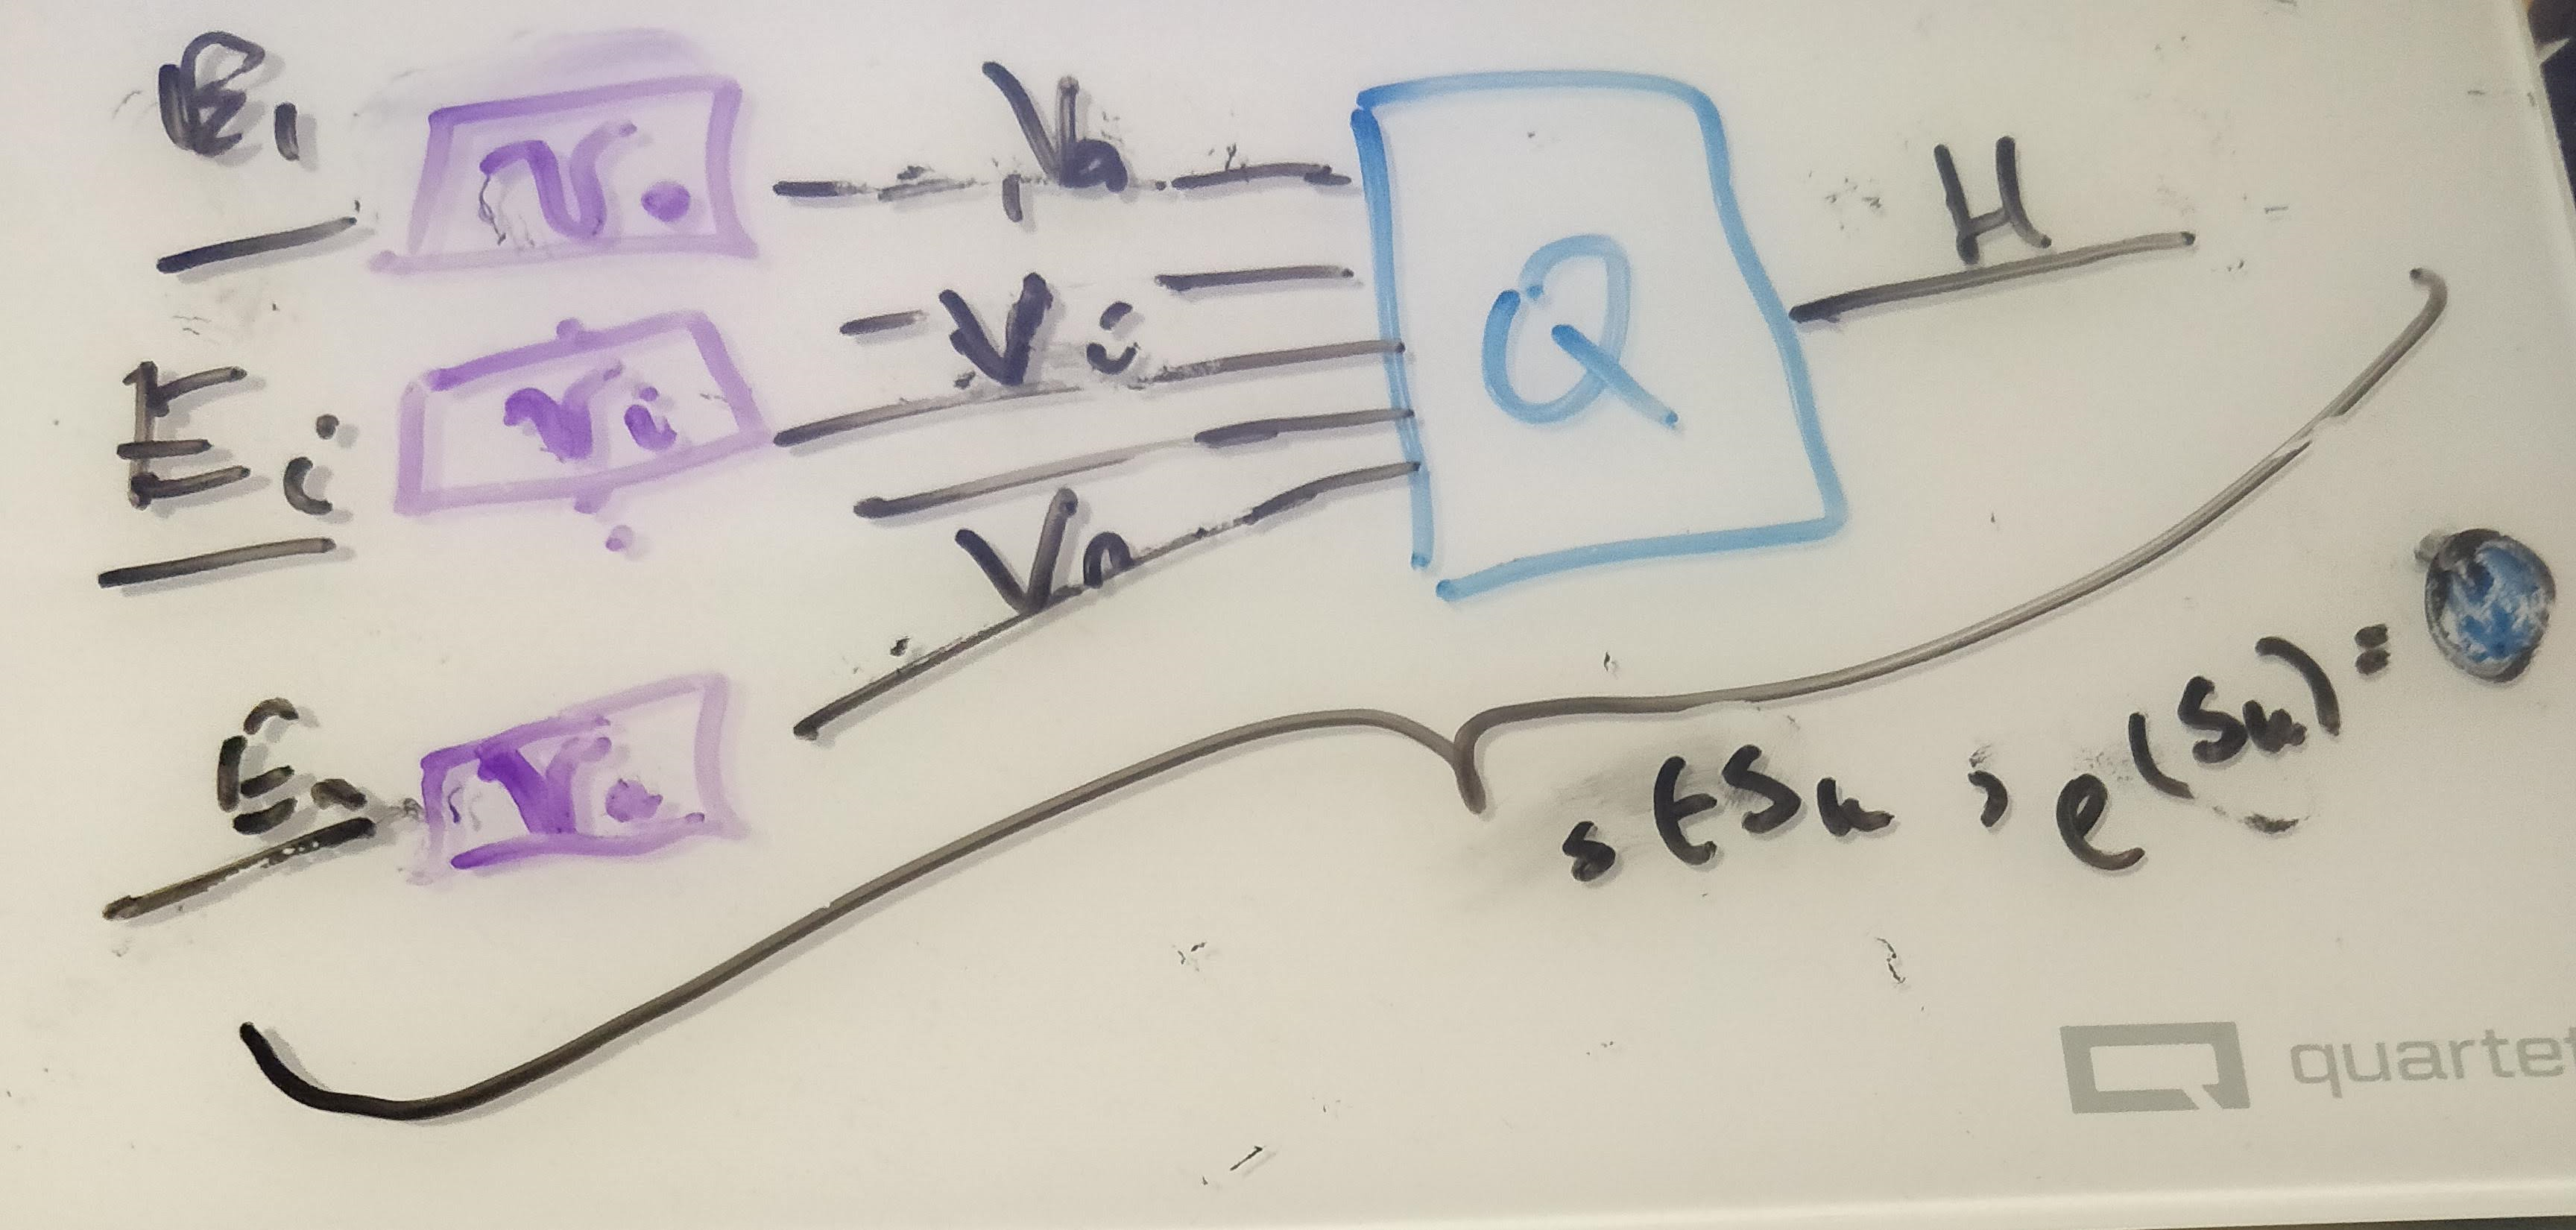
\includegraphics[width=\textwidth]{figures/math/path_of_q.png}
    \end{figure}
    \pause
    \begin{equation*}
        \label{eq:nu_expanded}
        \{\vchannel_{0}, \ldots, \vchannel_{n}\}: \{\dsection_{0}, \ldots, \dsection_{n}\} \mapsto \{\vsection_{0}, \ldots, \vsection_{n}\}
    \end{equation*}
    \pause
    \begin{equation*}
        Q = \nu \circ \tau
    \end{equation*}
\end{frame}


\begin{frame}{Stevens' Scales \cite{stevensTheoryScalesMeasurement1946}}
\begin{table}[H]
    \begin{tabularx}{\textwidth}{|l|l|X|}\toprule
        \textbf{scale} & \textbf{group} & \textbf{constraint} \\\midrule
        nominal & permutation &  $\text{if } \delement_1 \neq \delement_2 \text{ then } \vchannel (\delement_1) \neq\vchannel(\delement_2)$\\
        ordinal &  monotonic & $\text{if } \delement_1 \leq \delement_2 \text{ then } \vchannel (\delement_1) \leq \vchannel(\delement_2)$\\
        interval &  translation &  $\vchannel (x + c) = \vchannel(x) + c$ \\
        ratio &  scaling &  $\vchannel(xc) = \vchannel(x)*c $\\ \bottomrule
    \end{tabularx}
\end{table}
\end{frame}

\begin{frame}{Equivariance: Partial Order}
    \begin{figure} %break out steps/reveal
        \includegraphics[width=1\textwidth]{figures/math/monoid_equivariant.png}
    \end{figure}
\end{frame}


\begin{frame}{Visualization Equivariance}
    \begin{figure}[H]
        \includegraphics[width=\textwidth]{figures/math/diff_type_q.png}
    \end{figure}

    %put equation w/ rho, label rho, rho'
\end{frame}

\begin{frame}{Scatter: $\vmark(xpos, ypos)(\alpha, \beta)$}
    \begin{figure}[H]
        \includegraphics[width=1\textwidth]{figures/math/scatter.png}
    \end{figure}
    
    \begin{align*}
        x &= size *\alpha \cos(\beta) + xpos \\
        y &= size *\alpha \sin(\beta) + ypos
    \end{align*}    
\end{frame}

\begin{frame}{Line: $\vmark(xpos, \hat{n_{1}}, ypos, \hat{n_{2}})(\alpha, \beta)$ }
    \begin{figure}[H]
        \includegraphics[width=1\textwidth]{figures/math/line.png}
    \end{figure}
\end{frame}

\begin{frame}{Image $\vmark(xpos, ypos, color)$}
    \begin{figure}[H]
        \includegraphics[width=1\textwidth]{figures/math/image.png}
    \end{figure}
\end{frame}

\begin{frame}{Build \vmark over \dbase:\vmarkd}
\begin{figure}[H]
    \includegraphics[width=1\textwidth]{figures/math/q_hat.png}
\end{figure}
\begin{equation*}\label{eq:qhat_q_s}
    \vmarkd(\vsection(\dbasepoint))(\gbasepoint) \coloneqq \vmark((\vsectionpull)(\gbasepoint))
\end{equation*} 
such \gbasepoint\ can be factored out when $\vpreimg = \gbasepoint$
\end{frame}

\begin{frame}{Composition of artists} 
    % make disjointed figure or scatter + line
    Given the family of artists $(\dtotal_i: i\in I)$ on the same image
    \begin{equation*}
        + \coloneqq \underset{i\in I}{\sqcup} \dtotal_{i}
    \end{equation*}
    the + operator defines a simple composition of artists. 
\end{frame}


\section{Prototype}
\begin{frame}{TEAM driven rearchitecture of Matplotlib}
    \begin{itemize}
        \begin{itemize}
            \item topologically complex heterogenous data 
            \item target display spaces
        \end{itemize}
        \pause
        \item structure preserving maps from data to visual
            \begin{itemize}
                \item data and graphics have equivalent continuity
                \item properties are equivariant under monoid actions
            \end{itemize}  
        \pause
        \item composable into complex visualizations
    \end{itemize}
\end{frame}

\begin{frame}[fragile]{How do we make things with this model?}
    \begin{figure}[H]
        \begin{subfigure}{0.49\textwidth}
            \includegraphics[width=\textwidth]{figures/code/scatter_0.png}
        \end{subfigure}
        \begin{subfigure}{0.49\textwidth}
            \includegraphics[width=\textwidth]{figures/code/line_1.png}
        \end{subfigure}
    \end{figure}
    \begin{columns}
    \column{0.49\textwidth}
    \begin{minted}{python}
    fig, ax = plt.subplots()
    artist = Point(data, transforms)
    ax.add_artist(artist)
    \end{minted}
    \column{.49\textwidth}
    \begin{minted}{python}
    fig, ax = plt.subplots()
    artist = Line(data, transforms)
    ax.add_artist(artist)
    \end{minted}
    \end{columns}
\end{frame}

\subsection{Visual Transforms}
\begin{frame}[fragile]{How do we implement \vchannel?}
    \begin{minted}{python}
    cmap =  color.Categorical({'true':'deeppink', 'false':'deepskyblue'})
    transforms = {'x': {'name': 'v4', 'encoder': lambda x: x},
                    'y': {'name': 'v2', 'encoder': lambda x: x},
                    'facecolors': {'name':'v3', 'encoder': cmap}, 
                    's':{'name': None , 
                        'encoder': lambda _: itertools.repeat(.02)}}
    \end{minted}
    \begin{itemize}
        \item \mintinline{python}{lambda x: x} is identity \vchannel\
        \item \mintinline{python}|{'name':None}| map into \vfiber\ without corresponding \dsection\
        \item \mintinline{python}{color.Categorical} is custom \vchannel
    \end{itemize}
\end{frame}
    

\subsection{Artist}
\begin{frame}[fragile]{Artist} %% rewrite w/ letters in talk
    \begin{minted}{python}
        class ArtistClass(matplotlib.artist.Artist):
            def __init__(self, E, V, *args, **kwargs):
                # set properties that are specific to the artist
                # stash the input E and V
                super().__init__(*args, **kwargs)
        
            def qhat(self, **args):
                # set the properties of the graphic
        
            def draw(self, renderer):
                # returns tau, indexed on fiber then key 
                tau = self.E.view(self.axes) 
                # visual channel encoding applied fiberwise 
                visual = {p_i: nu_i(tau_i)
                          for p_i, nu_i, tau)i 
                          in zip(self.V, tau)}
                self.qhat(**visual)
                # pass configurations off to the renderer
                super().draw(renderer)
        \end{minted}
\end{frame}

\begin{frame}[fragile]{Artists: Scatter \& Line}
%%keep the signatures, comments, change names to math
\begin{minted}{python}
    class Point(mcollections.Collection):
        def assemble(self, x, y, s, facecolors='C0' ):
            # construct geometries of the circle glyphs in visual coordinates
            self._paths = [mpath.Path.circle(center=(xi,yi), radius=si) 
                        for (xi, yi, si) in zip(x, y, s)] 
            # set attributes of glyphs, these are vectorized 
            # circles and facecolors are lists of the same size
            self.set_facecolors(facecolors)

    class Line(mcollections.LineCollection):
        def assemble(self, x, y, color='C0'):
            # assemble line marks as set of segments 
            segments = [np.vstack((vx, vy)).T for vx, vy in zip(x, y)]
            self.set_segments(segments)
            self.set_color(color)
    \end{minted}
\end{frame}

\subsection{Data}
\begin{frame}[fragile]{Continuity}
    \begin{minted}{python}
class PointData: 
    # Fiberbundle is consistent across all sections
    FB = FiberBundle({'tables': ['vertex']},  
        {'v1': float, 'v2': str, 'v3': float})
    def tau(self, k):
        return # tau evaluated at one point k

class LineData: 
    FB = FiberBundle({'tables': ['edge']},
                {'x' : float, 'y':  float, 'color':mtypes.Color()})
    def tau(self, k): 
        return # tau evaluated on interval k
    \end{minted}
\end{frame}

\begin{frame}[fragile]{Same Artist, Different Data Configurations}
    \begin{figure}[H]
        \begin{subfigure}{0.49\textwidth}
            \includegraphics[width=\textwidth]{figures/code/linec_1.png}
        \end{subfigure}
        \begin{subfigure}{0.49\textwidth}
            \includegraphics[width=\textwidth]{figures/code/lined_1.png}
        \end{subfigure}
    \end{figure}
\begin{minted}{python}
LineData(FB, edge_table, vertex_table, connect=True)
LineData(FB, edge_table, vertex_table, num_samples=2, connect=False)
\end{minted}
\end{frame}

\begin{frame}{Proposed Dissertation}
% math + prototypes, organize it
% papers + contributions to matplotlib
\begin{itemize}
    \item expansion of the mathematical framework to include worked out simple and complex addition
    \item formalization of definition of equivalance class \vartisteq
    \item implementation of artist with explicit \vindex\
    \item specification of interactive visualization
    \item mathematical formulation of a graphic with axes labeling
    \item implementation of new prototype artists that do not inherit from Matplotlib artists
    \item provisional mathematics and implementation of user level composite artists
    \item proof of concept domain specific user facing library 
\end{itemize}
\end{frame}

\section{References}
\begin{frame}[allowframebreaks]{References}
\printbibliography
\end{frame}
\appendix 
\subsection{Appendix}

\end{document}

